\documentclass[journal,12pt,twocolumn]{IEEEtran}
\usepackage{amsthm}
\usepackage{graphicx}
\usepackage{mathrsfs}
\usepackage{txfonts}
\usepackage{stfloats}
\usepackage{pgfplots}
\usepackage{cite}
\usepackage{cases}
\usepackage{mathtools}
\usepackage{caption}
\usepackage{enumerate}	
\usepackage{enumitem}
\usepackage{amsmath}
\usepackage[utf8]{inputenc}
\usepackage[english]{babel}
\usepackage{multicol}
%\usepackage{xtab}
\usepackage{longtable}
\usepackage{multirow}
%\usepackage{algorithm}
%\usepackage{algpseudocode}
\usepackage{enumitem}
\usepackage{mathtools}
\usepackage{gensymb}
\usepackage{hyperref}
%\usepackage[framemethod=tikz]{mdframed}
\usepackage{listings}
    %\usepackage[latin1]{inputenc}                                 %%
    \usepackage{color}                                            %%
    \usepackage{array}                                            %%
    \usepackage{longtable}                                        %%
    \usepackage{calc}                                             %%
    \usepackage{multirow}                                         %%
    \usepackage{hhline}                                           %%
    \usepackage{ifthen}                                         %%
  \providecommand{\nCr}[2]{\,^{#1}C_{#2}}
  \providecommand{\nPr}[2]{\,^{#1}P_{#2}}
  \lstset{
%language=C,
frame=single, 
breaklines=true,
columns=fullflexible
}

\title{Assignment 2
\\Probability and Random Variables }
\author{Swati Mohanty (EE20RESCH11007) }
\date{September 2020}

\begin{document}

\maketitle


\section{Problem}
In a meeting, {70\%} of the members favour and {30\% }oppose a certain proposal. A member is selected at random and we take X = 0 if he opposed, and X = 1 if he is in favour. Find E(X) and Var (X).

\section{Solution}
A member opposes the proposal : X=0;\\
A member favours the proposal : X=1;\\
P(X=0) = 70 {\%} = 0.7\\
P(X=1) = 30 {\%} =0.3
\begin{align}
    E(X) = \sum_{i=1}^{n} x_i p_i 
    \\= 1\times0.7 + 0\times0.3 =0.7
    \\\implies E(X) =0.7
    \\E(X^2) = \sum_{i=1}^{n} (x_i)^2 p_i 
    \\= 1^2\times0.7 + 0^2\times0.3 =0.7
    \\Var(X) = E(X^2) -[E(X)]^2
    \\= 0.7- 0.7^2 = 0.21
    \\\implies Var(X) =0.21
\end{align}
\\The same  result is also obtained using the python code.
\begin{figure}[h]
\renewcommand{\theenumi}{1}
\centering
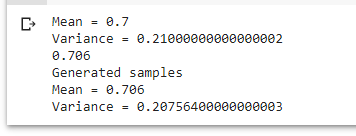
\includegraphics[ width=\columnwidth , height =3cm]{bern.png}
\caption{Result obtained from python code }
\label{Fig:1}
\end{figure}
\\\textbf{Download python code from here}\\
\begin{lstlisting}
https://github.com/Swati-Mohanty/AI5002/blob/main/Assignment%202/codes/bernoullidist.py
\end{lstlisting}
\\\textbf{Download latex code from here-}\\
\begin{lstlisting}
https://github.com/Swati-Mohanty/AI5002/blob/main/Assignment%202/codes/assignment2.tex
\end{lstlisting}

\end{document}
